\nsection{OSN 11 Метод нумерации значений в пределах базового блока и в пределах процедуры. Реализация метода путем построения ориентированных ациклических графов и использования хеш-таблиц.}

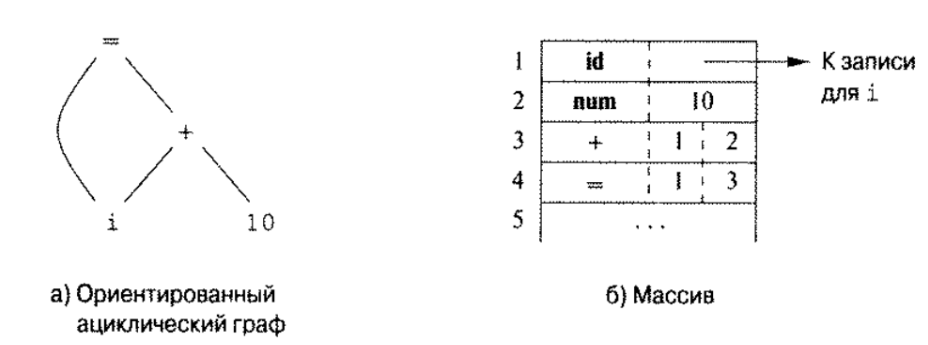
\includegraphics[width=\linewidth]{pics/graph_alg.png}

Зачастую узлы синтаксического дерева или ориентированного ациклического графа хранятся в массиве записей, как предложено на рис. 6.6. Каждая строка мас- сива представляет одну запись, а следовательно, один узел. Первое поле каждой записи представляет собой код операции, указывая метку узла. На рисунке в части б у листьев имеется по одному дополнительному полю, в котором хранится лексическое значение (указатель на запись в таблице символов или константа), а внутренние узлы имеют по два дополнительных поля, указывающих левый и правый дочерние узлы.

Мы обращаемся к узлам с использованием целочисленного индекса соответ- ствующей записи в массиве. Это целочисленное значение исторически носит на- звание номер значения (value number) узла или выражения, представленного этим узлом. Например, на рисунке узел с меткой + имеет номер значения 3, а номера значений его левого и правого дочерних узлов равны соответственно 1 и 2. На практике вместо целочисленных индексов можно использовать указатели на записи или ссылки на объекты, но мы в любом случае будем говорить о ссылке на узел как о "номере значения". Будучи сохраненными с применением подходящей структуры данных, номера значений помогают эффективно строить ориентированные ациклические графы.

Предположим, что узлы хранятся в массиве, как показано на рисунке, и что обратиться к каждому узлу можно по его номеру. Назовем сигнатурой внутренне- го узла тройку (ор,1,г), где ор - метка, 1 номер значения левого, a r - правого дочернего узла. Унарный оператор можно рассматривать как имеющий значение r = 0.

Алгоритм. 6.3 \textbf{Метод номера значения построения узла ориентированного ациклического графа}
\begin{itemize}
    \item ВХОД: метка ор, узлы l и r.
    \item ВЫХОД: номер значения узла с сигнатурой (ор, l, r) в массиве.
    \item МЕТОД: выполнить поиск в массиве узла М с меткой ор, левым дочерним узлом l и правым дочерним узлом г. Если такой узел найден, вернуть номер значения М. Если нет, создать в массиве новый узел N с меткой ор, левым дочерним узлом l и правым дочерним узлом г и вернуть его номер значения.
\end{itemize}

Хотя алгоритм 6.3 и выдает на выходе требуемую информацию, сканирование всего массива всякий раз, когда нам требуется получить информацию об одном узле, метод слишком расточительный, в особенности если в массиве хранятся выражения из всей программы. Более эффективный подход заключается в использовании хеш-таблицы, в которой узлы помещаются в блоки (buckets), в каждом из которых обычно хранится всего лишь несколько узлов. Хеш-таблица представляет собой одну из нескольких структур данных, эффективно поддерживающих словари.

Для построения хеш-таблицы для узлов ориентированного ациклического гра- фа требуется хеш-функция h, которая вычисляет индекс блока по сигнатуре (ор, l, г) способом, который равномерно распределяет сигнатуры по блокам, так что маловероятна ситуация, когда в одном блоке находится существенно больше узлов, чем в другом. Индекс блока h (op,l,r) детерминированно вычисляется на основании значений ор, l и г, так что сколько бы мы ни повторяли вычисления, для заданной тройки (ор, l, г) мы всегда будем получать один и тот же индекс.
Блоки могут быть реализованы в виде связанных списков, как показано на рисунке ниже. Массив, проиндексированный хеш-значениями, хранит заголовки блоков, каждый из которых указывает на первую ячейку списка. Внутри связанного списка блока каждая ячейка хранит номер значения одного из узлов, хешированных в данный блок, т.е. узел (ор, l, г) может быть найден в списке, заголовок которого имеет в массиве индекс h (op, l, r).

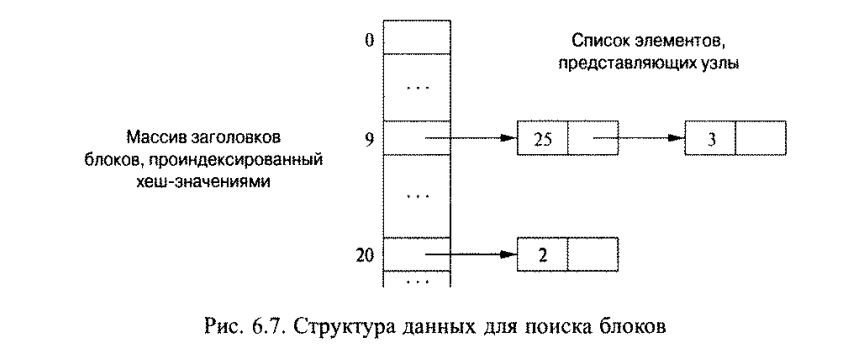
\includegraphics[width=\linewidth]{pics/hash_table_arg.png}

Таким образом, для данных ор, l и r мы вычисляем индекс блока h (op,l,r) и ищем заданный узел в списке ячеек этого блока. Обычно блоков достаточно для того, чтобы списки состояли всего лишь из нескольких узлов. Однако при поиске может потребоваться просканировать все ячейки блока, и для каждого номера значения и, найденного в ячейке списка, следует проверить соответствие сигнатуры искомого узла (ор,l,r) узлу в списке (как показано на рисунке выше). Если соответствие найдено, мы возвращаем и, если нет, то, поскольку нам известно, что в других блоках данный узел храниться не может, мы создаем новую ячейку, добавляем ее к списку ячеек блока с индексом h (op,l,r) и возвращаем номер значения этой новой ячейки.